\documentclass{scrartcl}
\usepackage[ngerman]{babel} % default Sprache für alles (Datum usw.)
\usepackage[affil-it]{authblk}
\usepackage{setspace} % Zeilenabstand
\usepackage{csquotes} % um ,,hello" zu benutzen
\usepackage[sorting=none]{biblatex} 
\usepackage[most]{tcolorbox} % Codeblocks
\usepackage{graphicx}
\usepackage[bottom]{footmisc}
\usepackage{booktabs}
\usepackage[normalem]{ulem} % strikethrough
\usepackage{makecell}
\DefineBibliographyStrings{ngerman}{ % u.a. -> et al.
   andothers = {et al\adddot}
}
\definecolor{gray}{rgb}{0.94, 0.94, 0.95}
\setlength{\parindent}{0pt} % Sets the paragraph indent to 0

\addbibresource{references.bib}

\begin{document}

\begin{titlepage}

   \subject{Literatur-Seminar-Arbeit}
   \title{Vorhersagen von Verkehrsunfällen mithilfe künstlicher neuronaler Netze}
   \author{Erik Rohr}
   \affil{Fachbereich Informatik (02) - Hochschule Bonn-Rhein-Sieg}
   \publishers{\parbox[b][12cm]{\textwidth}{\centering Betreuerin: Doerthe Vieten}}
   \date{\today}

   \maketitle

\end{titlepage}

\newpage
\onehalfspacing

\section*{Abstrakt}
$\ll$ Kurz beschreiben $\gg$

\newpage
\tableofcontents
\newpage

\section{Einleitung}

Jedes Jahr sterben weltweit ca. 1,19 Millionen Menschen in Verkehrsunfällen
(RTA, engl.: \enquote{road traffic accident}) \cite{who}.
Eine umfassende Analyse vorliegender Verkehrsdaten im Hinblick auf potentielle
Bedrohungen kann dazu beitragen, Baumaßnahmen unfallminimierend zu gestalten.
\medskip \\
Vorangehende Analysen von Verkehrsdaten, die eine Vielzahl an \enquote{Machine Learning}
-Modelle nutzten, haben ergeben, dass eine Vielzahl an Faktoren existieren,
die das Risiko auf RTA erhöhen, wie Wetterbedingungen, Straßenkonditionen,
Zustand des Fahrers, Lichtverhältnisse, Tageszeit und die Verkehrsdichte \cite{das, qian}.
\enquote{Machine Learning}-Modelle (ML) sind darauf ausgelegt, nicht anhand von
spezifischen Anweisungen, sondern allein durch das Erkennen von Mustern und
Abhängigkeiten mithilfe komplexer Funktionen \cite{qian} in Daten Erkenntnisse
zu ziehen und Entscheidungen sowie Vorhersagen treffen zu können \cite{sap}.
\medskip \\
Unter den ML-Modellen werden künstliche neuronale Netze (KNN) für diesen
Anwendungsfall bevorzugt, da diese keine zugrundeliegenden Beziehungen
zwischen den Eingangsvariablen benötigen und darauf ausgelegt sind,
mit historischen Daten Vorhersagen zu tätigen \cite{qian}.
\medskip \\
In dieser Arbeit wird eine systematische Literaturrecherche (SLR) zur Vorhersage
von RTAs mithilfe KNNs dargestellt. Die Ergebnisse werden im Hinblick auf deren
Mehrwert in der Minimierung von Straßenverkehrsunfällen durch unsichere
Planung der Architektur untersucht und eingeordnet.

\subsection{Theorie}

Zunächst werden die theoretischen Grundlagen sowie die Forschungslage 
von KNN ausgeführt, um die Ergebnisse der Literaturrecherche in den 
Kontext einordnen zu können.

\subsubsection{Künstliche neuronale Netze (KNN)}
Künstliche neuronale Netze (KNN) sind ein Teilbereich der ML-Modelle. Sie können
Entscheidungen auf ähnlicher Art und Weise treffen, wie das menschliche Gehirn \cite{ibm}.
Das Modell besteht aus einer Vielzahl von Schichten mit unterschiedlich vielen
Knoten. Diese Knoten sind mit anderen Knoten aus den benachbarten Schichten verbunden
und besitzen sogenannte \enquote{weights} und \enquote{bias} \cite{ibm}.
Eingabedaten werden von der \enquote{input layer} (Deutsch: \enquote{Eingangsschicht})
entlang aller hidden layer (Deutsch: \enquote{verborgene Schicht}) durchgereicht,
verarbeitet und schließlich in der \enquote{output layer}
(Deutsch: \enquote{Ausgangsschicht}) aggregiert ausgegeben \cite{ibm}.
\medskip \\
Zur Konfigurierung von KNN können unter anderem die Anzahl der Schichten,
die Optimierungsverfahren (engl.: \enquote{optimizers}) (OV), die
Aktivierungsfunktion (engl.: \enquote{activation function}) (AF) und die
Verlustsfunktion (engl.: \enquote{loss function}) frei gewählt werden
\cite{actopt}.
\medskip \\
Ein Optimierungsverfahren ist eine Funktion oder ein Algorithmus, welches
die Gewichte der Knoten und die Lernrate (engl.: \enquote{learning rate})
anpasst, um den Verlust zu minimieren, die Genauigkeit zu maximieren und
die benötigte Trainingszeit exponentiell zu reduzieren \cite{actopt}.
Beispiele für solche Optimierungsverfahren sind der \enquote{gradient descent},
\enquote{RMS prop (Root Mean Square)} und \enquote{adam's optimizer} \cite{actopt}.
\smallskip \\
Die AF entscheidet, wie der kalkulierte Ausgangswert
eines Knotens zu interpretieren ist. Dies fügt dem Netz eine Nicht-Linearität
hinzu \cite{actopt}. Somit können die verborgenen Schichten jeweils für
andere Bereiche der Interpretation der Daten stehen. Linearität würde auf
der anderen Seite bedeuten, dass das Netz in eine Funktion zusammengefasst
werden könnte \cite{actopt}. Beispiele sind die binäre \enquote{step function},
die Sigmoid-Funktion und die \enquote{RELU}-Funktion \cite{actopt}.
\smallskip \\
Eine Verlustsfunktion (VF) misst, wie genau das KNN den Datensatz modelliert, indem
es den vorliegenden Verlust (engl.: \enquote{loss}) berechnet \cite{actopt}.
Gängige Funktionen sind die \enquote{Mean Squared Error}-Funktion und die
\enquote{Binary Cross Entropy}-Funktion \cite{actopt}.

\subsection{Historische Forschungslage}

\subsubsection{Smith et al.}
Die Anwendung eines neuronalen Netzes ist an einer Simulation einer
\enquote{nine intersection} in Manhattan, New York untersucht worden.
Es ergab sich eine 10-prozentige Verringerung in der Wartezeit von Fahrzeugen
im Vergleich zur Nutzung der bereits existierenden, \enquote{in-place} Strategie \cite{smith}.

\subsubsection{Edmond Chin-Ping Chang}
Die Anwendung von einem neuronalen Netz auf \enquote{traffic engineering} wird mithilfe 
verschiedener Sensoren und historischer Daten erforscht. Die Effektivität wird mit
einem konventionellen Algorithmus verglichen und anschließend werden zwei neuronale Netze
trainiert, um die Herangehensweisen beider Mittel zu kombinieren (\cite{chang} S. 642).
Man hat herausgefunden, dass trotz dem Verlust geringfügiger Genauigkeit das Zwei-Neuronale-Netz-Modell
sehr geeignet für das Verarbeiten von Verkehrsunfallsdaten ist (\cite{chang} S. 645).

\subsection{Aktuelle Forschungslage}

\subsubsection{Banerjee et al.}
Eine Vielzahl an Klassifizierern (engl.: \enquote{classifiers}) sind mit
KNN-Modellen bezüglich Vorhersage der Mortalität in RTAs verglichen worden.
Darunter gehören
Random Forest, Support Vector Machine, K-Nearest Neighbor Classifier,
AdaBoost Classifier, XGBoost Classifier. Hierbei hat das KNN mit 7
\enquote{hidden layer}, 1 \enquote{input layer}, Adams Optimizer und einer
\enquote{dropout class} in der Eingangsschicht die beste Genauigkeit von 84,36\%
erzielt \cite{akt1}.

\subsubsection{Maurya et al.}
Vorhersehen von Kraftfahrzeuggeschwindigkeiten dienen als Basis für ein
fortgeschrittenes Verkehrsmanagementsystem \cite{akt2}. Hierbei wurden
Lineare Regression, \enquote{random forest}-Regression, \enquote{Decision Tree} und
ein KNN miteinander Vergleichen uns eine \enquote{Performance Analyse} durchgeführt.
KNN und die \enquote{random forest}-Regression haben mit einem
\enquote{R squared}-Wert \footnote{Bestimmtheitsmaß.
   Stellt die Anpassungsgüte einer Regression dar \cite{rsquared}}
von jeweils 0,9301 und 0,9642 das beste Fitting erzielt \cite{akt2}.

\subsubsection{Zohra et al.}
Anhand den Datensätzen aus \enquote{US Accidents (2016-2023)} wurden ein KNN,
ein Random Forest Klassifizierer und eine logistische Regression trainiert und
getestet. Hier wurden jeweils Genauigkeitswerte von 81,1\%, 90,7\% und 87,03\%
erreicht \cite{akt3}.

\section{Methodik}
Im Folgenden wird die Vorgehensweise bei der Literaturrecherche beschrieben.
Die Vorgehensweise orientert sich an der PRISMA-Leitlinie (Preferred Reporting
Items for Systematic Reviews and Meta-Analyses). PRISMA hat sich ursprünglich
als effektiver Vorreiter bzgl. SLR im medizinischen Sektor etabliert, mit dem
Fachkräfte auf dem aktuellen Stand der Wissenschaft bleiben und bestehende
Vorschriften aktualisiert werden \cite{prisma}. Entnehmend der zahlreichen
SLR-Veröffentlichungen in Bereichen der Informatik (siehe Datenbanken ACM/IEEE),
hat sich PRISMA als hilfreiches Mittel zur SLR auch in anderen
Wissenschaftsbereichen bewiesen und wird daher als Instrument der SLR
in dieser Arbeit verwendet.

\subsection{Die PRISMA-Leitlinie}
PRISMA beinhaltet eine aus 27 Stichpunkten bestehende \enquote{Checkliste}
und ein 4-phasiges Fluss-Diagramm \cite{prisma}. Da diese allerdings ursprünglich
für die Medizin entwickelt wurden, werden jene auf die Informatik angepasst
als Basis der SLR verwendet.  Mithilfe dieser Elemente kann sowohl Literatur
systematisch für die Aufnahme in einer SLR auf Eignung geprüft als auch der
Prozess erleichtert und standardisiert werden.
\medskip \\
Zunächst werden Forschungsfragen aufgestellt, die im Laufe der Recherche beantwortet
werden sollen. Im Anschluss wird dann die Literatur anhand der ausgewählten
Such-Strategie ausgewählt. Die gesammelte Literatur wird dann durch Ein- und
Ausschlusskriterien auf Eignung für die SLR durch die Checkliste geprüft.
Schließlich werden aus der eingeschlossenen Literatur qualitative und quantitative
Daten extrahiert, mit anderer Literatur verglichen und in der eigentlichen
Literaturanalyse zusammengetragen.

\subsection{Forschungsfragen}

Um die Literaturrecherche zu systematisieren, werden laut PRISMA \cite{prisma}
Forschungsfragen aufgestellt, damit ein systematisches Full-Text-Screening für
die Eignung möglich ist. In Rahmen dieser Arbeit wurden folgende Fragen aufgestellt:
\begin{enumerate}
   \item{ Welche Netztopologie sind verwendet worden? }
   \item{ Welche Genauigkeit konnte erzielt werden? }
   \item{ Wie viele Knoten sind in den verborgenen Schichten verwendet worden?}
   \item{ Wie ist der Lernprozess realisiert worden? (\enquote{optimizer}, \enquote{loss function} usw.) ?}
   \item{ Welche Eingabevariablen sind gewählt worden?}
\end{enumerate}

\subsection{In- und Exklusionskriterien}
Um gezielt die Potenz künstlicher neuronaler Netze für die Verkehrsanalyse zu
untersuchen, sind spezifische Ein- und Ausschlusskriterien gewählt worden. Somit
wird die Anzahl der aus der Suche ergebenen Artikel reduziert und verschafft
einen besseren Überblick.

Die für diese Arbeit relevanten Artikel sind auf solche beschränkt worden, die
\begin{enumerate}
   \item{eine Verkehrsdatenanalyse untersuchen und die Daten mit einer KNN auswerten,}
   \item{ggf. einen quantitativen Vergleich verschiedener ML-Modelle durchführen oder}
   \item{quantitative Merkmale der KNN aufzählen.}
\end{enumerate}
Zu letzterem Punkt gehören Merkmale wie gewählte Netztopologie, Anzahl der Schichten,
Anzahl der Knoten pro Schicht, gewähltes Optimierungsverfahren, die gewählte
AF Genauigkeit und Eingangsvariablen.

\subsection{Prozess der Recherche}

Für die Literaturrecherche sind die Datenbanken ACM Digital Library und die
IEEE Explore verwendet worden, da diese überwiegend Artikel in der Informatik
veröffentlicht haben.
Hierbei wurden die folgenden Suchstrings verwendet:

\begin{tcolorbox}[
      enhanced,
      attach boxed title to top left,
      colback=gray!20,
      colframe=gray,
      colbacktitle=gray,
      title=ACM Digital Library,
      fonttitle=\bfseries\color{black},
      boxed title style={size=small, colframe=gray, sharp corners},
      sharp corners
   ]
   [All: "neural network?"] AND [ [All: "traffic flow"] OR [All: "traffic control"] OR [All: \dq accident"] ] AND [E-Publication Date: (01/01/2023 TO 12/31/2024)]
\end{tcolorbox}

\begin{tcolorbox}[
      enhanced,
      attach boxed title to top left,
      colback=gray!20,
      colframe=gray,
      colbacktitle=gray,
      title=IEEE Explore,
      fonttitle=\bfseries\color{black},
      boxed title style={size=small, colframe=gray, sharp corners},
      sharp corners
   ]
   (\dq All Metadata\dq: \dq artificial neural network?")
   AND (\dq All Metadata":"traffic")
   AND (\dq All Metadata":"control\dq\space
   OR \dq All Metadata":\dq accident")
\end{tcolorbox}

Bei der \enquote{IEEE-Explore}-Datenbank wurde als Zeitraum-Filter der 01.01.2023
bis zum 31.12.2024 gewählt, da dieser nicht in den Such-String mit eingebunden
werden konnte.  Zusätzlich ist die Suche auf den Inhaltstyp
\enquote{Research Article} und die Verfügbarkeit \enquote{Open Access}
begrenzt worden, soweit von den Einstellungen beider Datenbanken möglich.
\medskip \\
Die zusammengetragenen Artikel wurden im Anschluss mithilfe des PRISMA
Fluss-Diagramms \cite{prisma} auf Eignung überprüft (Abb. \ref{abb1}) und in einer Tabelle
zusammengefasst (Tab. \ref{tab1}).

\begin{figure}[h!]
   \centering
   \caption{SLR nach PRISMA}
   \label{abb1}
   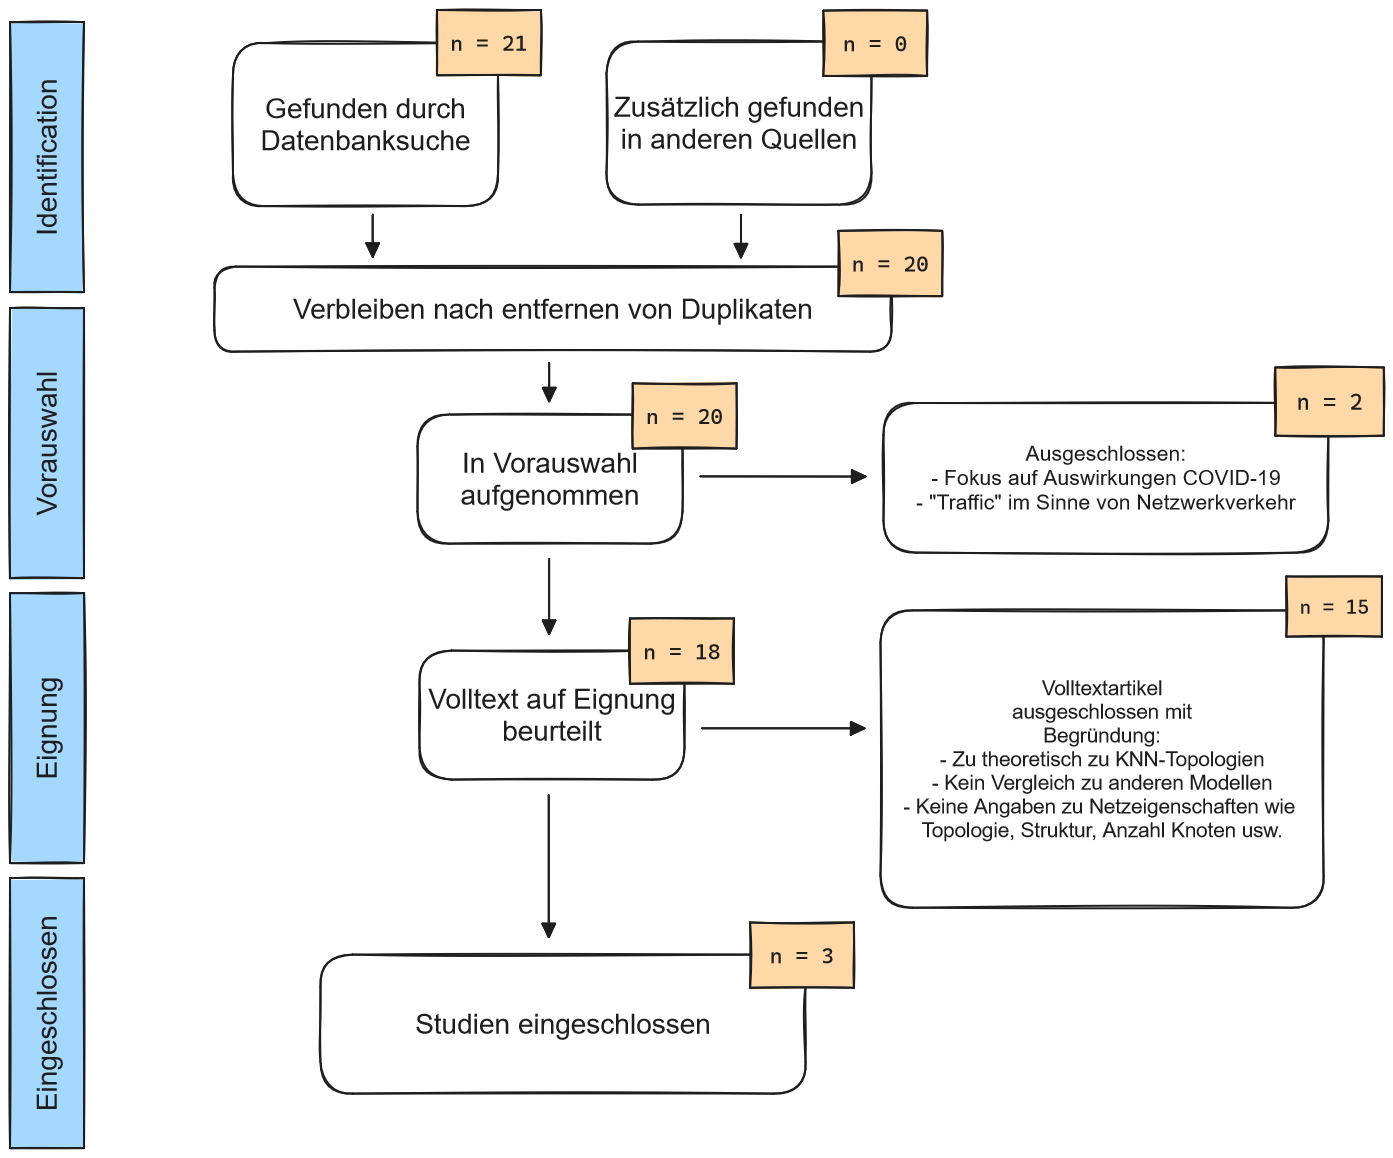
\includegraphics[scale=0.28]{Bilder/prisma-exported.png}
\end{figure}

\section{Ergebnisse}

\subsection{Qian et al.}

Qian et al. haben eine Kombination aus einem \enquote{classification and regression trees} (CART)
und einem \enquote{back propagation neural network} (BPNN) entwickelt und mit einer 
logistischen Regression, AdaBoost und dem naiven Bayes Klassifizierern verglichen.
Die Untersuchung ergab, dass das CART-BPNN-Modell mit einer Genauigkeit von 78,56\% 
am besten abschnitt \cite{qian}.

\subsection{Das et al.}
In dieser Studie sind verschiedene KNN-Modelle verschieden-parametrisiert verglichen worden.
Hierbei wurden Modelle mit unterschiedlichen OVs und AFs trainiert und ausgewertet. 
Das Modell mit einer Softmax-AF und Adams Optimierungsverfahren erzielte die höchste
Genauigkeit von 94,62\% \cite{das}.

\subsection{Bao et al.}
Ein KNN mit einer und zwei verborgenen Schicht(en), allerdings mit einer insgesamt
gleichbleibenden Anzahl an verborgenen Knoten, sind miteinander verglichen worden.
Der Vergleich ergab, dass zwar das Modell mit zwei Schichten geringfügig besser abschnitt
als das Modell mit einer Schicht, allerdings um mehr als das 20-fache an Trainingszeit
benötigte. Daher ist man zum Schluss gelangt, dass eine verborgene Schicht für diesen
Anwendungsfall besser geeignet ist.


\begin{table}[h!]
   \centering
   \caption{Ergebnisse der Literaturrecherche}
   \begin{tabular}{lccc} \toprule
      Autoren         & Qian et al. \cite{qian} & Das et al.  \cite{das} & Bao et al. \cite{bao} \\ \midrule
      Topologie       & BPNN                    & FFNN                   & BPNN                  \\
      AF              & Softmax                 & Softmax                & Sigmoid               \\
      VF              & Cross-Entropy           & Cross-Entropy          & Levenberg Marquardt   \\
      Verborg. Knoten & $3$                     & o.A.                   & $388$                 \\
      Lernrate        & 0.01                    & o.A.                   & 0,005                 \\
      OV              & Gradient Descent        & Adam                   & o.A.                  \\
      Genauigkeit     & 78,56\%                 & 94,62\%                & 69,95\%               \\
      \bottomrule
   \end{tabular}
   \label{tab1}
   \medskip \\
   {\raggedright \textit{Anmerkung: \enquote{o.A.} = \enquote{ohne Angabe}} \par}
\end{table}
\begin{table}[h!]
   \centering
   \caption{Eingabevariablen der KNN-Modelle}
   \begin{tabular}{lc} \toprule
      Autoren & Eingabevariablen \\ \midrule
      Qian et al. & \makecell[r]{Minute, Stunde, Jahr, Monat, Tag, Polizeieinsatz, Gebietsart, \\ Fahrbahngefahren, Straßensonderbedingungen, \\ Straßenoberflächenbedingungen, Wetterbedingungen, Lichtverhältnisse, \\ Fußgängerüberweg vorhanden, Straßennummer und -Klasse, \\ Krezungsverwaltung, Geschwindigkeitsbegrenzung, Straßentyp, \\ Wochentag, Anzahl Verunglückte, \\ Anzahl Fahrzeuge, Längen- und Breitengrad} \\ \midrule
      Das et al. & \makecell[r]{Jahreszeit, Fahrzeugart des Unfallbeteiligten, Gebietsart, \\ Aufprallart, Unfallsart, Alter des Beteiligten \\ \enquote{a.m. peak}, \enquote{a.m. off-peak}, \enquote{p.m. peak}, \enquote{p.m. off-peak}} \\ \midrule
      Bao et al. & \makecell[r]{Kreuzungsart, Unfallsortsart, Straßentyp, \\ Mittelstreifenart, Nicht-verkehrsbezogene Mittelstreifenart, \\ Straßenmaterial, Straßenkonditionen, Bürgersteigkonditionen, \\ Lichtverhältnisse, Wetterbedingungen, Sichtweite, Unfallsart} \\ \bottomrule
   \end{tabular}
   \label{tab2}
\end{table}

Die Ergebnisse der Studien fallen sehr unterschiedlich aus. Sowohl Qian et al.
als auch Das et al. beführworten die Nutzung von KNN in der Durchführung
und Auswertung von Verkehrsanalysen (\cite{qian} S. 2744, \cite{das} S. 5),
allerdings empfielt Bao et al., dass zukünftige Studien sich intensiver mit
den einzelnen Faktoren der Verkehrsanalyse befassen sollten, da Verkehrsanalysen
zu komplex sind, diese in einem Modell zusammenzufassen (\cite{bao} S. 784).
\medskip \\
Diese Rückschlüsse werden auch von den erreichten Genauigkeiten der KNN-Modelle
reflektiert: Absteigend sortiert erreichte Das et al. eine Genauigkeit von 94,62\%, Qian et al. 78,56\%
und von Bao et al. einer Genauigkeit von 69,95\% \cite{das, qian, bao}.
\medskip \\
Entnehmend der Tabelle \ref{tab1} gibt es dennoch einige Gemeinsamkeiten
zwischen den Studien. Sowohl Qian et al. als auch Bao et al. verwendeten für
ihre Netztopologie ein BPNN
(\cite{qian} S. 2739, \cite{bao} S. 782), wohingegen Das et al. als besten Kandidat
ein \enquote{feed forward neural network} (FFNN) nominierte (\cite{das} S. 2).
Bezüglich den Aktivierungs- und Verlustsfunktionen verwenden Qian et al.
und Das et al. jeweils die Softmax-AF und die Cross-Entropy-VF
(\cite{qian} S. 2742, \cite{das} S. 2).
Bao et al. haben hier hingegen eine Sigmoid-Funktion als AF und den
\enquote{Levenberg Marquardt}-Algorithmus als VF verwendet (\cite{bao} S. 783).
Sowohl in der gewählten Lernrate, dem gewählten Optimierungsverfahren und den
gewählten Eingabevariablen unterscheiden sich die drei Studien maßgeblich.
Qian et al. nutzten 3 verborgene Knoten mit einer Lernrate von 0,01, während
Bao et al. 388 verborgene Knoten (\cite{bao} S. 783) und eine Lernrate von 0,005 
für ihre Analysen verwendeten. 
Das et al. hat zu beiden Attributen keine Werte angegeben.
\medskip \\
Der Tabelle \ref{tab2} entnehmend sind die Eingabevariablen der Modelle divers.
Qian et al, Das et al. und Bao et al. haben hierbei jeweils 31, 6 und 12 
verschiedene Variablen für ihre Modelle gewählt.

\section{Diskussion und Fazit}

Im Rahmen der SLR werden im Folgenden die Ergebnisse der Studien kritisch untersucht,
Limitationen sowohl der Studien als auch dieser SLR aufgezeigt und zusätzlich
zum Fazit eine Empfehlung für zuküftige Forschungen im Bereich der Verwendung
von KNN für Verkehrsanalysen ausgesprochen.

\subsection{Diskussion}

Alle drei inkludierten Studien sind zu maßgeblich unterschiedlichen Ergebnissen
auf unterschiedlichen Wegen gekommen. Das et al. und Bao et al. stechen
mit Genauigkeiten von jeweils 94,62\% und 69,95\% aus den Rechercheergebnissen
heraus. Im Rahmen einer Verkehrsanalyse sollten die verwendeten Modelle so
zuverlässig wie möglich sein, allerdings besteht die Gefahr, dass das trainierte
Modell einem sog. \enquote{over-fitting} (OF) oder \enquote{under-fitting} (UF)
unterliegt. OF bezeichnet eine zu starke Anpassung des Modells an die Trainingsdaten,
weswegen es neue Daten nicht korrekt auswertet \cite{aws}.
Dies kann unter anderem passieren, falls die Trainingsdaten für den gewählten
Klassifizierungskontext irrelevante Datensätze beinhalten
(auch genannt \enquote{verrauschte Daten}), die Größe der Trainingsdaten
zu klein, oder die Parameter des Modells zu komplex
gewählt worden sind \cite{aws}. Das Pendant dazu ist ein Vorliegen eines UF.
Hierbei ist das Modell zu simpel und kann Muster dementsprechend nicht auffassen
und verinnerlichen \cite{ibm2}.
\medskip \\
Bao et al. erreichte auf dem Testdatensatz eine Genauigkeit von 69,95\% mit
einem \enquote{1-Hidden-Layer}-Modell. Im Gegensatz zu diesem Datensatz
erreichte dieses Modell
eine Genauigkeit von 76,1\% auf den Trainingsdaten (\cite{bao} S. 784).
Es ist anzunehmen, dass das Modell mit 388 verborgenen Knoten zu
komplex gewählt und daher einem OF unterliegen könnte.
Im Vergleich dazu erreichten Das et al. eine Genauigkeit von 94,62\%.
Die hohe Differenz zu den anderen beiden Studien liegt vermutlich in der Tatsache,
dass das Modell auf einer kleineren Menge an Eingabevariablen trainiert wurde
(siehe Tabelle \ref{tab2}). Hierbei haben Das et al. mit 10 Eingabevariablen
die wohl simpelste Eingangsschicht gewählt. Vergleichsweise haben Bao et al. zwei mehr und
Qian et al. das Dreifache an Eingangsvariablen verwendet, wodurch die Komplexität der
Modelle ansteigt \cite{aws}.
\medskip \\
Aussagen über die gewählte Netztopologie im Bezug auf die Genauigkeitsdifferenz
können aufgrund fehlender Angaben von Das et al. nicht getroffen werden. Es ist unklar,
wie Das et al. die verborgene(n) Schichten konfiguriert haben.
Das et al. haben eine relativ ähnliche Konfiguration gewählt wie Qian et al., allerdings
mehr als 16\% höhere Genauigkeit erziehlen können.
Durch diese Ähnlichkeiten ist unklar, ob die Eingangsvariablen
oder die Gestaltung der verborgenen Schichten des KNN bedeutender für die Genauigkeit nach
dem Training der Modelle sind.
\medskip \\
Bao et al. erläutert, dass ihr Modell aufzeigt, dass die gewählten Eingangsvariablen zu
komplex gewählt wurden und weitere Forschung diesbzgl. benötigt sei (\cite{bao} S. 784), lässt allerdings die
gewählten Netz-Topologie-Parameter außer acht in dieser Ausführung. Interessant wäre zu wissen,
wie die Netze mit unterschiedlichen Anzahlen von verborgenen Knoten abschneiden.

\subsection{Limitationen}

In dieser Arbeit werden lediglich drei Studien verglichen und eignet sich daher
nicht, eine allgemeingültige Aussage über die Legitimität künstlicher neuronaler
Netze im Bezug auf Verkehrsdatenanalyse zu treffen. Außerdem wurden nur
Artikel im Zeitraum vom 01.01.2023 bis zum 01.05.2024 betrachet, weswegen nur ein 
kleiner Einblick in die Forschung bereitet werden konnte.
\medskip \\
Aufgrund der beschränkten Anzahl der Artikel konnten außerdem keine Aussage
über neuere Netztopologien getroffen werden.

\subsection{Fazit}

Alle drei Studien beführworten die Verwendung von KNN in
Verkehrsdatenanalysen, um die Verkehrsplanung sicherer gestalten zu können
und dem überliegenden Ziel der Verkehrssicherheit einen Schritt näher zu kommen.
Qian et al. verglichen zusätzlich KNN-Modelle mit anderen
Regressionsmodellen und kamen zum Schluss, dass KNNs die zuverlässigste
Art von ML-Modellen ist, um mit historischen Daten Vorhersagen zu tätigen.
\medskip \\
Allerdings besteht bis heute die Herausforderung, optimale Parameter von
KNN angepasst auf die Verkehrsanalyse ausfindig zu machen und effektiv einzusetzen.

\subsection{Ausblick auf zukünftige Forschung}

Es wird empfohlen, näher auf die Parameter der gewählten KNN-Topologien
einzugehen und im Falle eines Vergleichs verschiedener Modelle diese auch
ausführlich auszuführen. Zukünftige Forschung sollte zusätzlich neuere
Topologien erforschen, wünschenswert auch eigenständige Modelle entwickeln.

\printbibliography
\listoffigures
\listoftables

\end{document}